\section{Literature Review}
\label{sec:bg-litreview}

    \subsection{Mosquito Wingbeat}
    \label{subsec:bg-litreview-mozz}
        
        Early research carried out by \textcite{Landois1866} in 1866 concluded that the flight tone of an insect was due to the number of wing strokes per second, otherwise known as the fundamental frequency or wingbeat of a flying insect. This set the basis for standard practises of determining flight tone by matching a tuning fork to the wingbeat by ear, a method lacking accuracy and objectivity. Only when \textcite{Williams1950} came along was it understood that the frequency components of an insect's wingbeat are of a more complex nature than a single tone and in fact are arranged in a harmonic structure. In a study conducted by \textcite{Belton1979} in 1979 on thirteen species of Canadian mosquito, it was found that wingbeat frequencies of each species overlapped but were distinct to at least five other species, and three species were distinct from nine others. However, there was no presence of an overlap between a female and male of the same species. 
        
        Recent research suggests that wingbeat alone, as a scalar, is not adequate to differentiate between mosquito species as there are more than 3,500 species of mosquito with wingbeats mostly in the range of 100-1000Hz \cite{Chen2014}. That range leaves 900Hz to describe 3,500 species, or 0.26Hz per species. This is not sufficient considering wingbeats per species can vary as much as 80Hz either way \cite{Arthur2014}. The use of audio features beyond that of the location of the first harmonic, as well as continuous audio capture of individual species, leads to high volumes of data which substantial information can be extracted from, aiding in this difficult challenge. Figure \ref{fig:bg-litreview-mozz-fft} shows the spectral components of the wingbeat of four species of mosquito, where both male and female specimens have been included for one species. The figure shows clear spectral overlap between classes, making species and gender classification a difficult challenge. The primary focus of this report is to detect mosquitoes over background noise with inexpensive sensors, although species discrimination of the resultant detection pipeline is also be tested using other sets of data.
        %  concern - each sample treated as i.i.d so training over continuous flight of a mosquito will make the classifier broadly detect over lots of frequencies, need to test first     
        % \textcite{Taylor1974} made a surprising discovery in a preceding study that one species (\textit{A. vexans}) would only mate in a cage if another species was present (\textit{A. dorsalis}). \textcite{Belton1979} were able to measure the wingbeat frequencies of both and found that median values were within 5Hz of each other, implying that the sound of the female \textit{dorsalis} may have stimulated the male \textit{vexans} to mate. This research proved that flying insect behaviour, particularly mosquitoes, is governed by sound, among other factors.
        \begin{figure}
            \centering
            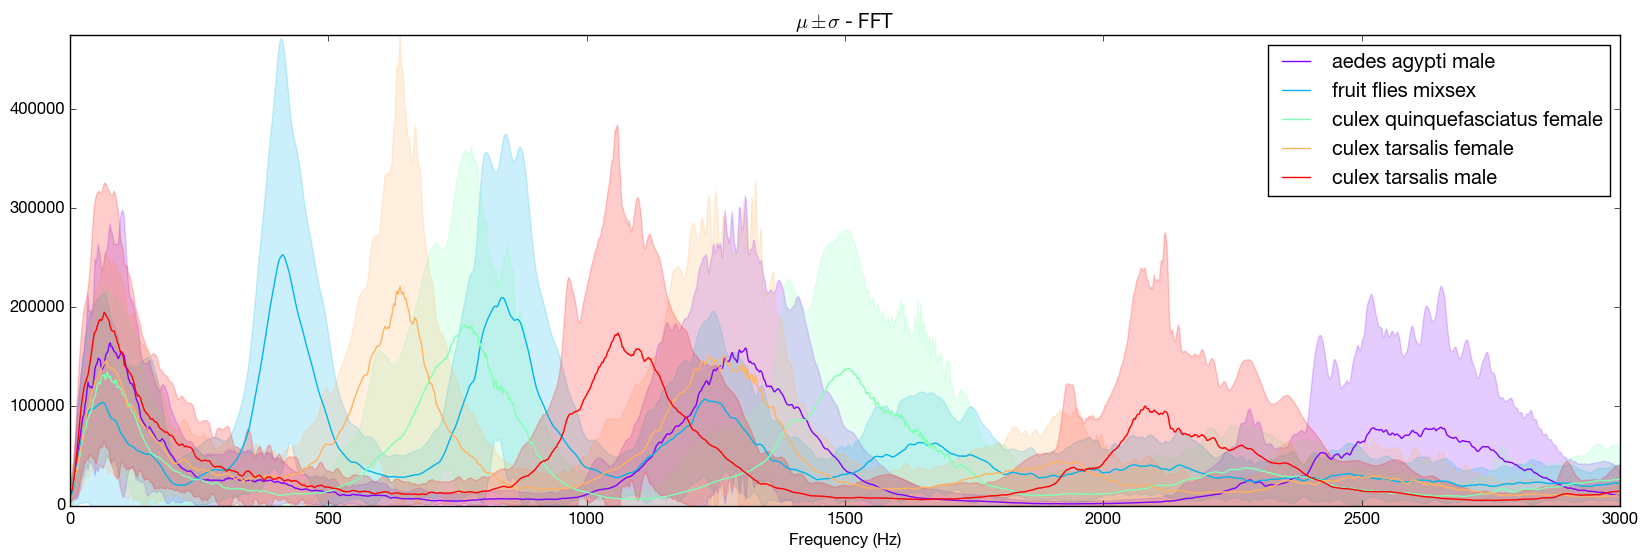
\includegraphics[width=\textwidth]{fft}
            \caption{FFT of four mosquito species, one including both male and female where the sample size is 500 specimens \cite{Chen2014}.}
            \label{fig:bg-litreview-mozz-fft}
        \end{figure}


    
    \subsection{Current Algorithms}
    \label{subsec:bg-litreview-currentalgs}
        \begin{sitemize}
            \item{come back to this later}
            \item{algorithms already applied in this context}
            \item{some papers saved in mendeley}
            \item{eg ivan NN + wavelet, shuyu AR, others saved in mendeley}
        \end{sitemize}
    
    % \subsection{Machine Learning}
    % \label{subsec:bg-litreview-machlearn}
    %     \begin{itemize}
    %         \item{introduce machine learning in general context}
    %     \end{itemize}